\documentclass[a4paper,english,12pt]{article}
\usepackage{%
	amsmath,%
	amsfonts,%
	amssymb,%
	amsthm,%
	hyperref,%
	url,%
	latexsym,%
	epsfig,%
	graphicx,%
	psfrag,%
	subfigure,%	
	color,%
	tikz,%
	pgf,%
	pgfplots,%
	pgfplotstable,%
	pgfpages,%
	proofs%
}

\usepgflibrary{shapes}
\usetikzlibrary{%
  arrows,%
	backgrounds,%
	chains,%
	decorations.pathmorphing,% /pgf/decoration/random steps | erste Graphik
	decorations.text,%
	matrix,%
  positioning,% wg. " of "
  fit,%
	patterns,%
  petri,%
	plotmarks,%
  scopes,%
	shadows,%
  shapes.misc,% wg. rounded rectangle
  shapes.arrows,%
	shapes.callouts,%
  shapes%
}

\theoremstyle{plain}
\newtheorem{thm}{Theorem}[section]
\newtheorem{lem}[thm]{Lemma}
\newtheorem{prop}[thm]{Proposition}
\newtheorem{cor}[thm]{Corollary}

\theoremstyle{definition}
\newtheorem{defn}[thm]{Definition}
\newtheorem{conj}[thm]{Conjecture}
\newtheorem{exmp}[thm]{Example}
\newtheorem{assum}[thm]{Assumptions}

%\theoremstyle{remark}
\newtheorem{rem}{Remark}
\newtheorem{note}{Note}

\makeatletter
\def\th@plain{%
  \thm@notefont{}% same as heading font
  \itshape % body font
}
\def\th@definition{%
  \thm@notefont{}% same as heading font
  \normalfont % body font
}
\makeatother
\date{}


\title{Lecture 17: Continuous Functions}
\author{}


\begin{document}
\maketitle

\section{Continuous Functions}
Let $(X,\T_X)$ and $(Y,\T_Y)$ be topological spaces. 
\begin{defn}[Continuous Function] A function $f:X\to Y$ is said to be \textbf{continuous} if the inverse image of every open subset of $Y$ is open in $X$. In other words, if $V\in \T_Y$, then  its inverse image $f^{-1}(V)\in \T_X$.
\end{defn}

\begin{prop}
A function $f:X\to Y$ is continuous iff for each $x \in X$ and each neighborhood $N$ of $f(x)$ in $Y$, the set $f^{-1}(N)$ is a neighborhood of $x$ in $X$.
\end{prop}
\begin{proof}
Let $x$ be an arbitrary element of $X$ and $N$ an arbitrary neighborhood of $f(x)$ in $Y$. Then, $f^{-1}(N)$ and contains $x$ and by definition, is open in $X$. Hence, for each $x \in X$ and each neighborhood $N$ of $f(x)$ in $Y$, the set $f^{-1}(N)$ is a neighborhood of $x$ in $X$.
Conversely, let for each $x \in X$ and each neighborhood $N$ of $f(x)$ in $Y$, the set $f^{-1}(N)$ is a neighborhood of $x$ in $X$. Let $V$ be an arbitrary open subset of $Y$. 
\begin{enumerate}[i)]
\item If $V\cap f(X)=\emptyset$, where $f(X)$ is the range of $f$, then $f^{-1}(V)=\emptyset$ and hence is open in $X$.
\item If $V\cap f(X)\neq \emptyset$, then $V$ is a neighborhood of each of its points (let $f(x)$ be one such point for some $x\in X$). By assumption, $f^{-1}(V)$ $(\subseteq X)$ must be a neighborhood of each of its points (including the said $x$) in $X$ and hence, $f^{-1}(V)$ is open in $X$.
\end{enumerate}
\end{proof}

\begin{note} Continuity of a function depends not only on $f$ but also on its domain and co-domain topologies $X$ and $Y$.
\end{note}

\begin{exmp}
Let $(X,\T_X)$ and $(Y,\T_Y)$ be topological spaces and $f:X\to Y$ be a function.
\begin{enumerate}[i)]
\item If $f$ is a constant map, \emph{i.e.}, $f(x)=y$ for all $x\in X$ and some $y\in Y$, then $f$ is continuous for all topologies on $X$ and $Y$ because for any open subset $V$ of $Y$, $f^{-1}(V)=\emptyset$ (if $y\notin V$) or $X$ (if $y\in V$), both of which are always open in any topology on $X$.
\item If $\T_X=\mathcal{P}(X)$, \emph{i.e.}, $(X,\T_X)$ is the discrete topology, then $f$ is continuous for any topology on $Y$ because for any open subset $V$ of $Y$, $f^{-1}(V)$ is in $\mathcal{P}(X)$ and hence is open in $X$.
\item If $\T_Y=\{\emptyset,Y\}$, \emph{i.e.}, $(Y,\T_Y)$ is the trivial topology, then $f$ is continuous for any topology on $X$ because $f^{-1}(\emptyset)=\emptyset$ and $f^{-1}(Y)=X$, both of which are always open in any topology on $X$.
\item The identity mapping from $(X,\T_X)$ to $(X,\T_X)$ is continuous because for any $U\in \T_X$ (co-domain topology), $f^{-1}(U)=U\in \T_X$ (domain topology).
\end{enumerate}
\label{many_ex}
\end{exmp}

\begin{exmp}
\item Let $(X,\T_X)$ and $(Y,\T_Y)$ be topological spaces defined as follows: 
\begin{equation*}
X=\{R,G,B\} \qquad \T_X=\{\emptyset,\{R\},\{B\},\{R,G\},\{R,B\},X\}
\end{equation*}
\begin{equation*}
Y=\{1,2,3\} \qquad  \T_Y=\{\emptyset,\{1\},\{1,2\},Y\} \qquad \qquad \qquad
\end{equation*}
Let $f$ and $g$ be bijective mapping defined as $f(R)=1$, $f(G)=2$ and $f(B)=3$. Then, $f$ is continuous since 
\begin{equation*}
f^{-1}(\emptyset)=\emptyset, \; f^{-1}(\{1\})=\{R\}, f^{-1}(\{1,2\})=\{R,G\}, \; f^{-1}(Y)=X 
\end{equation*}
all of which are open in $X$. However, its inverse map $g$, with $g(1)=R$, $g(2)=G$ and $g(3)=B$, is not continuous since 
\begin{equation*}
g^{-1}(\{B\})=\{3\}\notin \T_Y \text{ and } \; g^{-1}(\{R,B\})=\{1,3\}\notin \T_Y.
\end{equation*}
\label{inv_discont}
\end{exmp}

\begin{exmp}
The unit step function $u:\mathbb{R}\to \{0,1\}$ is given by 

  \begin{minipage}{.5\textwidth}
	\begin{equation*}
	u(x)= \begin{cases}
			0 \quad \text{if $x<0$}\\
			1 \quad \text{if $x\geqslant 0$}.
			\end{cases}
	\end{equation*}
  \end{minipage}%
  \begin{minipage}{.25\textwidth}
    \centering
    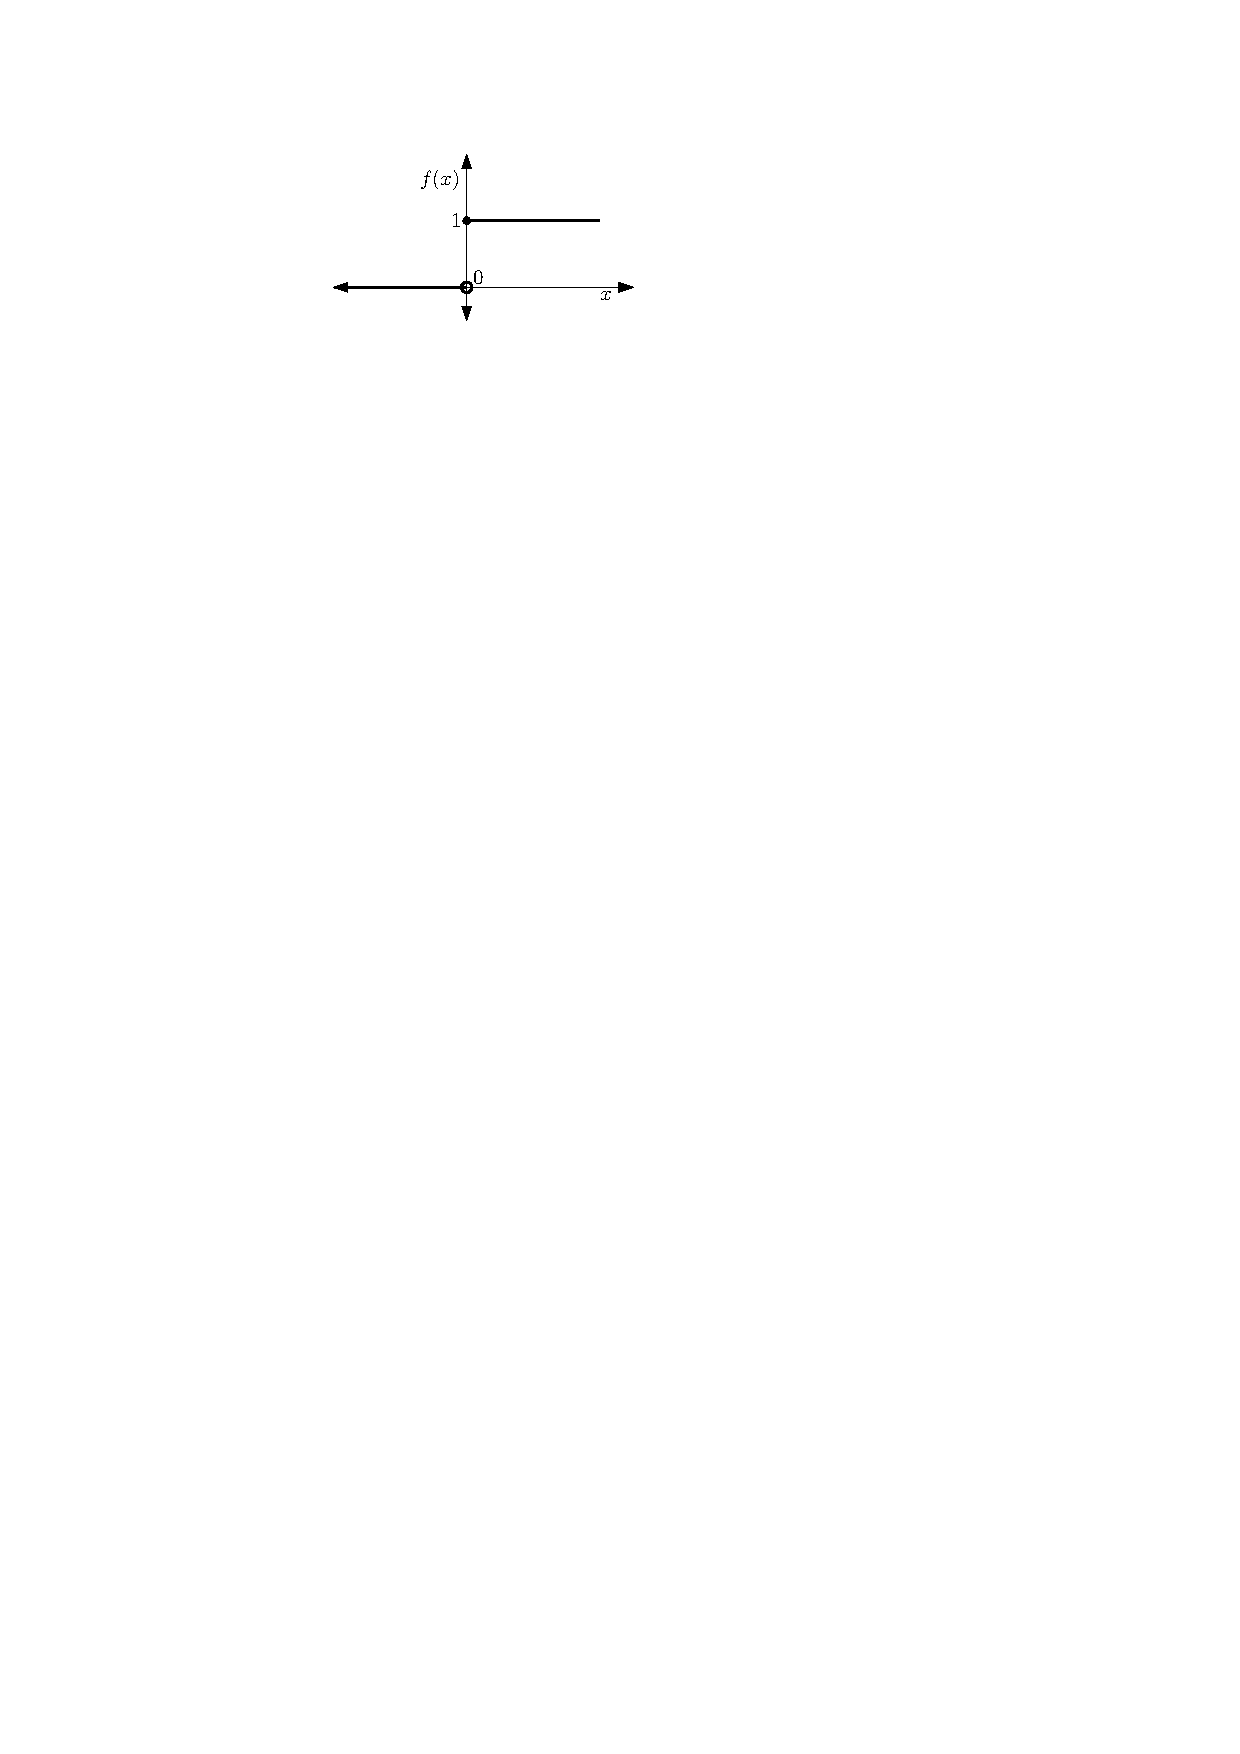
\includegraphics[scale=0.7]{Figures/step.pdf}
  \end{minipage}
  
\noindent Let $\mathbb{R}$ be equipped with the standard topology, \emph{i.e.}, all open intervals are open, and the set $\{0,1\}$ be equipped with the discrete topology. Then, $u^{-1}(0)=(-\infty,0)$ is open in the standard topology on $\mathbb{R}$, but $u^{-1}(1)=[0,\infty)$ is not. Hence, the unit step function is discontinuous.
\end{exmp}

\begin{exmp}
Let $\mathbb{R}$ and $\mathbb{R}_l$ denote the set of real numbers equipped with the standard and lower limit topology respectively, and $f:\mathbb{R}\to \mathbb{R}_l$ and $g:\mathbb{R}_l\to \mathbb{R}$ be identity functions, \emph{i.e.}, $f(x)=g(x)=x$, for every real number $x$. Then, $f$ is not continuous because the inverse image of the open set $[a,b)$ in $\mathbb{R}_l$ is $[a,b)$ which is not open in the standard topology. But $g$ is continuous because the inverse image of open interval $(a,b)$ in the standard topology on $\mathbb{R}$ is open in $\mathbb{R}_l$ ($g^{-1}((a,b))=(a,b)=\cup _{n\in \mathbb{N}}[a+\!^1/_n,b)$ and countable union of open sets is open).
\label{lower_lt}
\end{exmp}

\begin{exmp}
A function $f:\mathbb{R}\to \mathbb{R}$ is said to be continuous at $x_0\in \mathbb{R}$ if 
\begin{equation*}
\forall\,\epsilon>0,\,\exists\,\delta>0 \text{ such that } |x-x_0|<\delta\;\to\;|f(x)-f(x_0)|<\epsilon,
\end{equation*}
where both the domain and co-domain topologies are the standard topology on $\mathbb{R}$. The equivalence of this definition of continuity to the open-set definition of continuity at $x_0$ is shown below.

Let $f$ be continuous at $x_0$ by the open set definition, \emph{i.e.}, inverse image of every open set containing $x_0$ is open. Given any $\epsilon>0$, the interval $V=(f(x_0)-\epsilon,f(x_0)+\epsilon)$ is open in the co-domain topology and hence, $f^{-1}(V)$ is open in the domain topology. Since $f^{-1}(V)$ contains $x_0$, it contains a basis $(a,b)$ about $x_0$ (since for every open set $S$ and every $s\in S$, there exists a basis $B_s$ such that $s\in B_s\subseteq S$). Let $\delta$ be minimum of $x_0-a$ and $b-x_0$. Then if $|x-x_0|<\delta$, $x$ must be in $(a,b)$ and $f^{-1}(V)$ (since $(a,b)\subseteq f^{-1}(V)$). Hence $f(x)\in V$ and $|f(x)-f(x_0)|<\epsilon$ as required.

Now, let $f$ be $\epsilon-\delta-$continuous at $x\in \mathbb{R}$ and $V$ be an open set in the co-domain topology containing $f(x)$. Since $V$ is open and $f(x)\in V$, there exists some $\epsilon>0$, such that $(f(x)-\epsilon,f(x)+\epsilon)\subseteq V$. By continuity at $x$, there exists some $\delta>0$ such that $(x-\delta,x+\delta)\subseteq f^{-1}(V)$. Since $(x-\delta,x+\delta)$ is open in the domain topology and the choices of $\epsilon$ and $V$ were arbitrary, inverse image of every open set containing $x$ is open as required by the open set definition of continuity at $x$. Note that if an open set $V$ in co-domain topology does not intersect the range of $f$, then $f^{-1}(V)=\emptyset$, which is open in the domain topology. 
\end{exmp}

Following are some properties of continuity.
\begin{enumerate}
\item For two topologies $\T_X$ and $\T'_X$ on $X$, the identity map $1_X$ from $(X,\T_X)$ to $(X,\T'_X)$ is continuous iff $\T_X$ is finer than $\T'_X$.
\begin{proof}
Let $f=1_X$. Since the map is identity, $f^{-1}(S)=S$ for any subset $S$ of $X$. Let the identity map be continuous. Then, for any $V$ in $\T'_X$, $f^{-1}(V)$ is in $\T_X$. Since $f^{-1}(V)=V$, this means that $V$ is also in $\T_X$. Thus, $\T'_X\subseteq \T_X$, \emph{i.e.}, $(X,\T_X)$ is finer than $(X,\T'_X)$.
Conversely, let $\T_X$ is finer than $\T'_X$. Then, any set $S$ in $\T'_X$ is also in $\T_X$. For any $V$ in $\T'_X$, $f^{-1}(V)$ is in $\T_X$ because $f^{-1}(V)=V$ and $V$ is in $\T_X$. Thus, the identity map is continuous.
\end{proof}

\item A continuous map remains continuous if the domain topology becomes finer or the co-domain topology becomes coarser.
\begin{proof}
Let $(X,\T_1)$, $(X,\T_2)$, $(Y,\mathcal{S}_1)$ and $(Y,\mathcal{S}_2)$ be topologies with $\T_1$ and $\mathcal{S}_1$ finer than $\T_2$ and $\mathcal{S}_2$ respectively. Let $f$ be a continuous map from $(X,\T_2)$ to $(Y,\mathcal{S}_1)$. 
\begin{enumerate}[i)]
\item Let $V$ be in $\mathcal{S}_1$. Then, $f^{-1}(V)$ is in $\T_2$, since $f$ is continuous, and in $\T_1$, since it is finer than $\T_2$. Thus, $f$ is also a continuous map from $(X,\T_1)$ to $(Y,\mathcal{S}_1)$.
\item Let $V$ be in $\mathcal{S}_2$. Since, $\mathcal{S}_1$ is finer than $\mathcal{S}_2$, it contains $V$. Also $\T_2$ contains $f^{-1}(V)$ since $f$ is a continuous. Thus, $f$ is also a continuous map from $(X,\T_2)$ to $(Y,\mathcal{S}_2)$.
\end{enumerate}
\end{proof}

\end{enumerate}

\begin{note} \begin{enumerate}[i)]
\item From Property 1, it can be inferred that, continuity of a bijective function $f:X\to Y$ does not guarantees continuity of its inverse (cf. Examples~\ref{inv_discont} and \ref{lower_lt}).
\item In Example~\ref{lower_lt}, had $f$ been the identity map from $\mathbb{R}$ to itself then it would have been continuous but replacing the co-domain topology with a finer topology ($\mathbb{R}_l$) renders it discontinuous.
\end{enumerate} 

\end{note}

To test the continuity of a map from a topological space on $X$ to that on $Y$, checking whether inverse image of each open set in $Y$ is open in $X$ is not necessary.
\begin{thm}
Let $(X,\T_X)$ and $(Y,\T_Y)$ be topological spaces and $f:X\to Y$ be a function. Then, the following statements are equivalent:
\begin{enumerate}
\item $f$ is continuous.
\item Inverse image of every basis element of $\T_Y$ is open.
\item Inverse image of every subbasis element of $\T_Y$ is open.
\end{enumerate}
Thus, to test the continuity of a function it suffices to check openness of inverse images of elements of only a subset of $\T_Y$, \emph{viz.}, its subbasis.
\label{bas}
\end{thm}
\begin{proof}
\begin{description}
\item[(1)$\to$(2)]Let $f$ be continuous. Since every basis element of $\T_Y$ is open, its inverse image will be open.
\item[(2)$\to$(1)]Let $\mathcal{B}_Y$ be a basis for $\T_Y$ and let the inverse image of every basis element $B\in \mathcal{B}_Y$ be open in $X$, \emph{i.e.}, $f^{-1}(B)\in \T_X$. Note that any open set $V$ in $Y$ can be written as a union of the basis elements, \emph{i.e.}, $V=\cup _{j\in J}B_j$, $f^{-1}(V)=\cup _{j\in J}f^{-1}(B_j)$, for some $\{B_1,\dots,B_{|J|}\}\subseteq \mathcal{B}_Y$. Since union of opens sets is open, $f^{-1}(V)$ is open.
\item[(2)$\to$(3)]Since every subbasis element is in the basis it generates, inverse image of every subbasis element of $Y$ is open in $X$.
\item[(3)$\to$(2)]Let $\mathcal{S}_Y$ be subbasis of $Y$ which generates the basis $\mathcal{B}_Y$. Let the inverse image of every subbasis element $S\in \mathcal{S}_Y$ be open in $X$, \emph{i.e.}, $f^{-1}(S)\in \T_X$. Since any basis element can be written as a finite intersection of subbasis elements, \emph{i.e.}, $B=\cap _{i=1}^{n}S_i$, $f^{-1}(B)=\cap _{i=1}^{n}f^{-1}(S_i)$. Since finite intersection of open sets is open, $f^{-1}(B)$ is open in $X$.
\end{description}
\end{proof}

\begin{thm}
Let $f$ be a map from a topological space on $X$ to a topological space on $Y$. Then, the following statements are equivalent:
\begin{enumerate}
\item $f$ is continuous.
\item Inverse image of every closed set of $Y$ is closed in $X$.
\item For each $x\in X$ and every neighborhood $V$ of $f(x)$, there is a neighborhood $U$ of $x$ such that $f(U)\subseteq V$.
\item For every subset $A$ of $X$, $f(\overline{A})\subseteq \overline{f(A)}$.
\item For every subset $B$ of $Y$, $\overline{f^{-1}(B)}\subseteq f^{-1}(\overline{B})$.
\end{enumerate}
\end{thm}
\begin{proof}
\begin{description}
\item[(1)$\to$(2)]Let a subset $C$ of $Y$ be closed. Then, its complement $Y\backslash C$ is open and the inverse image of the complement $f^{-1}(Y\backslash C)=f^{-1}(Y)\backslash f^{-1}(C)=X\backslash f^{-1}(C)$ is open in $X$. Hence, $f^{-1}(C)$ is closed in $X$.
\item[(2)$\to$(1)]Let $V$ be open in $Y$. Then, its complement $Y\backslash V$ is closed and the inverse image of the complement $f^{-1}(Y\backslash V)=f^{-1}(Y)\backslash f^{-1}(V)=X\backslash f^{-1}(V)$ is closed in $X$. Hence, $f^{-1}(V)$ is open in $X$.
\item[(1)$\to$(3)]Since $f^{-1}(V)$ is an open neighborhood of $x$, choose $U=f^{-1}(V)$.
\item[(3)$\to$(4)]Let $A\subseteq X$ and $x\in \overline{A}$. Let $V$ be a neighborhood $f(x)$ and $U$ be a neighborhood of $x$ such that $f(U)\subseteq V$. Since $x\in \overline{A}$, $U\cap A\neq \emptyset$ and hence $\emptyset\neq f(U\cap A)\subseteq f(U)\cap f(A)\subseteq V\cap f(A)$ (cf. Lecture~5, Theorem 2.3(vii)). Since the choice of $V$ neighborhood of $f(x)$ was arbitrary, every neighborhood of $f(x)$ intersects $f(A)$. Hence, $f(x)\in \overline{f(A)}$ and $f(\overline{A})\subseteq \overline{f(A)}$.
\item[(4)$\to$(5)]Let $A=f^{-1}(B)$. Then, by (4), $f(\overline{A})\subseteq \overline{f(A)}=\overline{f(f^{-1}(B))}=\overline{B}$. Hence, $\overline{f^{-1}(B)}\subseteq f^{-1}(\overline{B})$.
\item[(5)$\to$(2)]Let $B\subseteq Y$ be closed; then, $\overline{B}=B$ since a set is closed iff it is equal to its closure. Then, by (5), $\overline{f^{-1}(B)}\subseteq f^{-1}(B)$ and since $f^{-1}(B)\subseteq \overline{f^{-1}(B)}$ is always true, $\overline{f^{-1}(B)}=f^{-1}(B)$. Hence, $f^{-1}(B)$ is closed (being equal to its closure).
\end{description}

\end{proof}


\section{Homeomorphism}

\begin{defn}[Homeomorphism] Let $(X,\T_X)$ and $(Y,\T_Y)$ be topological spaces and $f:X\to Y$ be a bijection. If both $f$ and its inverse $f^{-1}:Y\to 
X$ are continuous, then $f$ is called a \textbf{homeomorphism}.
\end{defn}

The two spaces are said to be \textit{homeomorphic} and each is a \textit{homeomorph} of the other. If a map is a homeomorphism, then so is its inverse. Composition of any two homeomorphisms is again a homeomorphism.

The requirement the $f^{-1}$ be continuous means that for any $U$ open in $X$, its inverse image under $f^{-1}$ be open in $Y$. But since the inverse image of $U$ under $f^{-1}$ is same as the image of $U$ under $f$ (cf. Lecture~5, Remark 2(vi)), another way to define a homeomorphism is to say that it is a bijective map $f:X\to Y$ such that $f(U)$ is open iff $U$ is open. Thus, a homeomorphism is a bijection between $\T_X$ and $\T_Y$. Consequently, any property of $X$ expressed in terms of $\T_X$ (or the open sets), yields, via $f$, the corresponding property for $Y$. Such a property is called a \textit{topological property} of $X$. % Thus, homeomorphism is the counterpart of \textit{isomorphism} in topology.

Let $f:X\to Y$ be an injective continuous map and $Z=f(X)\subset Y$ be its range, considered as a subspace of $Y$. Then, the map obtained by restricting $Y$ to $Z$, $f':X\to Z$ is a bijection. If $f'$ happens to be a homeomorphism, then we say that $f:X\to Y$ is a \textit{topological imbedding}, or simply an \textit{imbedding}, of $X$ in $Y$.

\begin{exmp}
Let $\mathbb{R}$ be equipped with the trivial, standard or discrete topology. For every pair of real numbers $m$ and $c$, the function $f_{m,c}:\mathbb{R}\to\mathbb{R}$ defined by $f_{m,c}(x)=mx+c,\forall x\in\mathbb{R}$ is a homeomorphism.
\end{exmp}

\begin{exmp}\begin{enumerate}[i)]
\item The identity map from a topological space to itself is a homeomorphism (Example~\ref{many_ex}(iv)).
\item The map $f$ in Examples~\ref{inv_discont} and the map $g$ in\ref{lower_lt} are both continuous and bijective but not homeomorphic because their inverse maps are not continuous.
\end{enumerate}
\end{exmp}

\begin{exmp}
\begin{enumerate}[i)]
\item Two discrete spaces are homeomorphic iff there is a bijection between them, \emph{i.e.}, iff they have the same cardinality. This is true because every function on a discrete space is continuous, no matter the co-domain topology (Example~\ref{many_ex}(ii)). 
\item Two trivial topologies are homeomorphic iff there is a bijection between them. This holds because every function to a trivial topology is continuous regardless of the domain topology (Example~\ref{many_ex}(iii)). 
\end{enumerate}
\end{exmp}

\begin{prop} Let $(X,\T_X)$ and $(Y,\T_Y)$ be topological spaces and $f:X\to Y$ be a function. Then, the following statements are equivalent:
\begin{enumerate}[i)]
\item $f$ is a homeomorphism.
\item $U$ is open in $X$ iff $f(U)$ is open in $Y$.
\item $C$ is closed in $X$ iff $f(C)$ is closed in $Y$.
\item $V$ is open in $Y$ iff $f^{-1}(V)$ is open in $X$.
\item $D$ is closed in $Y$ iff $f^{-1}(D)$ is closed in $X$.
\end{enumerate}
\end{prop}

\section{Constructing Continuous Functions}
Some rules for constructing continuous functions are given below.

\begin{thm} Let $X$, $Y$ and $Z$ be topological spaces.
\begin{enumerate}
\item (Constant function) If $f:X\to Y$ defined as $f(x)=y$ for all $x\in X$ and some $y\in Y$, then $f$ is continuous.
\item (Inclusion) If $A$ is a subspace of $X$, then the inclusion function $j:A\to X$ is continuous. ($j(a)=a,\,\forall\,a\in A$)
\item (Composites) If $f:X\to Y$ and $g:Y\to Z$ are continuous, then so is their composition $g\circ f:X\to Z$.
\item (Restricting the domain) If $f:X\to Y$ is continuous and $A$ is a subspace of $X$, then the restriction of $f$ to $A$, $f|A:A\to Y$ is also continuous.
\item (Restricting or expanding the range) Let $f:X\to Y$ be continuous. 
		\begin{enumerate}[a)]
		\item If $Z$ is subspace of $Y$ containing the range $f(X)$, then the function $g:X\to Z$ obtained by restricting the co-domain topology is continuous.
		\item If $Z$ is space containing $Y$ as a subspace, then the function $h:X\to Z$ obtained by expanding the co-domain topology is continuous.
		\end{enumerate}
\item (Local formulation of continuity)The map $f:X\to Y$ is continuous if $X$ cna be written as the union of open sets $U_{\alpha}$ such that $f|U_{\alpha}$ is continuous for each $\alpha$.
\end{enumerate}
\label{rules}
\end{thm}
\begin{proof}
\begin{enumerate}[i)]
\item See Example~\ref{many_ex}(i).
\item If $U$ is open in $X$, then $j^{-1}(U)=U\cap A$ is open in $A$ by definition of subspace topology.
\item If $W$ is open in $Z$, then $g^{-1}(W)$ is open in $Y$ since $g$ is continuous. Since $f$ is continuous, $f^{-1}(g^{-1}(W))$ is open in $X$. Thus, $g\circ f$ is continuous (since $f^{-1}(g^{-1}(W))=(g\circ f)^{-1}(W)$).
\item $f|A=j\circ f$, both of which are continuous and composition of continuous maps is continuous.
\item (a) Let $W$ be open in $Z$. Then, $B=Z\cap U$ for some $U$ open in $Y$. Since $f(Z)\subseteq Z$, $f^{-1}(B)=f^{-1}(U)$ and is open in $X$ because $f^{-1}(U)$ is open in $X$.
(b) Let $j:Y\to Z$ be the inclusion map. Then, $h=f\circ j$.
\item Let $V$ be open in $Y$. Then, 
\begin{equation*}
f^{-1}(V)\cap U_{\alpha}=(f|U_{\alpha})^{-1}(V)
\end{equation*}
and is open in $U_{\alpha}$ and hence open in $X$. But 
\begin{equation*}
f^{-1}(V)=\bigcup _{\alpha}\left( f^{-1}(V)\cap U_{\alpha}\right),
\end{equation*}
so that $V$ is also open in $X$.
\end{enumerate}
\end{proof}

\begin{thm}[The Pasting Lemma]
Let $X=A\cup B$, where $A$ and $B$ are closed in $X$. Let $f:A\to Y$ and $g:B\to Y$ e continuous maps. If $f(x)=g(x)$ for every $x\in A\cap B$, the $f$ and $g$ combine to give a continuous map $h:X\to Y$, defined as 
\begin{equation*}
h(x)=\begin{cases} f(x) \quad \mathrm{if } \;\; x\in A \\ g(x) \quad \mathrm{if}\;\; x\in B.
\end{cases}
\end{equation*}
\end{thm}
\begin{proof}
Let $C$ be a closed subset of $Y$. Then, $h{-1}(C)=f^{-1}(C)\cup g^{-1}(C)$ and is closed in $X$ since each of $f^{-1}(C)$ and $g^{-1}(C)$ are closed in $X$.
\end{proof}

The pasting lemma hold even if $A$ and $B$ are open in $X$ and is a special case of Theorem~\ref{rules}(vi).

\begin{thm}[Maps into Products]
Let $f:A\to X\times Y$ be defined as $f(a)=(f_1(a),f_2(a))$. Then $f$ is continuous iff both the co-ordinate functions $f_1:A\to X$ and $f_2:A\to Y$ are continuous.
\end{thm}
\begin{proof}
The projection maps $\pi_1:X\times Y\to X$ and $\pi_2:X\times Y\to Y$ onto the first and second factor space are continuous since $\pi_1^{-1}(U)=U\times Y$ and $\pi_2^{-1}(V)=X\times V$ are open if $U$ and $V$ are open in $X$ and $Y$ respectively. Note that $f_1=\pi_1\circ f$ and $f_2=\pi_2\circ f$.
If $f$ is continuous, then so are $f_1$ and $f_2$ (composites of continuous functions).
Conversely, let $f_1$ and $f_2$ are continuous. Let $U\times V$ be a basis element of  $X\times Y$. A point $a$ is in $f^{-1}(U\times V)$ iff $f(a)\in U\times V$, \emph{i.e.}, iff $f_1(a)\in U$ and $f_2(a)\in V$. Hence, $f^{-1}(U\times V)=f^{-1}(U)\cap f^{-1}(V)$ and is open in $A$ since both $f^{-1}(U)$ and $f^{-1}(V)$ are open. Thus, since inverse image of every basis element is open, $f$ is continuous (by Theorem~\ref{bas}(2))
\end{proof}

\end{document}
